\documentclass[14pt]{extbook}
\usepackage{multicol, enumerate, enumitem, hyperref, color, soul, setspace, parskip, fancyhdr} %General Packages
\usepackage{amssymb, amsthm, amsmath, bbm, latexsym, units, mathtools} %Math Packages
\everymath{\displaystyle} %All math in Display Style
% Packages with additional options
\usepackage[headsep=0.5cm,headheight=12pt, left=1 in,right= 1 in,top= 1 in,bottom= 1 in]{geometry}
\usepackage[usenames,dvipsnames]{xcolor}
\usepackage{dashrule}  % Package to use the command below to create lines between items
\newcommand{\litem}[1]{\item#1\hspace*{-1cm}\rule{\textwidth}{0.4pt}}
\pagestyle{fancy}
\lhead{Progress Quiz 4}
\chead{}
\rhead{Version B}
\lfoot{6286-1986}
\cfoot{}
\rfoot{Fall 2020}
\begin{document}

\begin{enumerate}
\litem{
Solve the radical equation below. Then, choose the interval(s) that the solution(s) belongs to.\[ \sqrt{-45 x^2 - 14} - \sqrt{-53 x} = 0 \]\begin{enumerate}[label=\Alph*.]
\item \( x \in [0,0.62] \)
\item \( x \in [0.49,0.88] \)
\item \( x_1 \in [0, 0.62] \text{ and } x_2 \in [-0.07,0.98] \)
\item \( \text{All solutions lead to invalid or complex values in the equation.} \)
\item \( x_1 \in [-0.47, -0.35] \text{ and } x_2 \in [-1.8,-0.36] \)

\end{enumerate} }
\litem{
Choose the equation of the function graphed below.
\begin{center}
    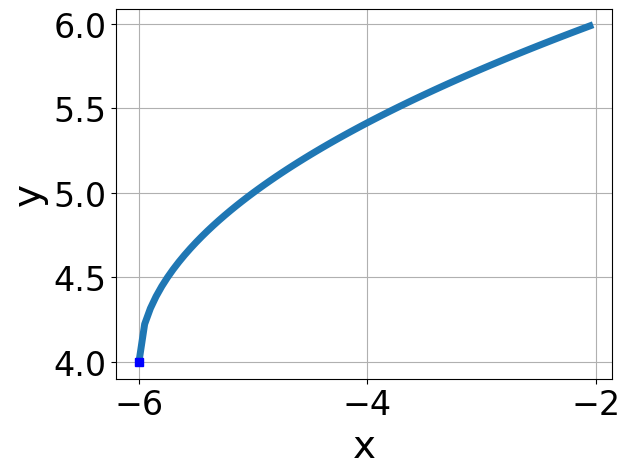
\includegraphics[width=0.5\textwidth]{../Figures/radicalGraphToEquationB.png}
\end{center}
\begin{enumerate}[label=\Alph*.]
\item \( f(x) = - \sqrt[3]{x - 10} + 3 \)
\item \( f(x) = - \sqrt[3]{x + 10} + 3 \)
\item \( f(x) = \sqrt[3]{x + 10} + 3 \)
\item \( f(x) = \sqrt[3]{x - 10} + 3 \)
\item \( \text{None of the above} \)

\end{enumerate} }
\litem{
Solve the radical equation below. Then, choose the interval(s) that the solution(s) belongs to.\[ \sqrt{81 x^2 + 40} - \sqrt{-117 x} = 0 \]\begin{enumerate}[label=\Alph*.]
\item \( x_1 \in [0.54, 0.7] \text{ and } x_2 \in [-0.3,2.7] \)
\item \( x \in [-0.65,-0.55] \)
\item \( \text{All solutions lead to invalid or complex values in the equation.} \)
\item \( x \in [-0.93,-0.6] \)
\item \( x_1 \in [-0.93, -0.6] \text{ and } x_2 \in [-1.7,0.4] \)

\end{enumerate} }
\litem{
Solve the radical equation below. Then, choose the interval(s) that the solution(s) belongs to.\[ \sqrt{-6 x - 2} - \sqrt{-7 x - 9} = 0 \]\begin{enumerate}[label=\Alph*.]
\item \( x \in [11,16] \)
\item \( x_1 \in [-10, -6] \text{ and } x_2 \in [-2.33,2.67] \)
\item \( x_1 \in [-3.29, 0.71] \text{ and } x_2 \in [-2.33,2.67] \)
\item \( \text{All solutions lead to invalid or complex values in the equation.} \)
\item \( x \in [-10,-6] \)

\end{enumerate} }
\litem{
What is the domain of the function below?\[ f(x) = \sqrt[6]{7 x + 8} \]\begin{enumerate}[label=\Alph*.]
\item \( (-\infty, a], \text{where } a \in [-1.87, -0.95] \)
\item \( (-\infty, \infty) \)
\item \( [a, \infty), \text{where } a \in [-1.02, -0.56] \)
\item \( [a, \infty), \text{ where } a \in [-1.34, -0.98] \)
\item \( (-\infty, a], \text{where } a \in [-0.94, -0.62] \)

\end{enumerate} }
\litem{
What is the domain of the function below?\[ f(x) = \sqrt[4]{7 x + 6} \]\begin{enumerate}[label=\Alph*.]
\item \( (-\infty, a], \text{where } a \in [-1.72, -1.11] \)
\item \( [a, \infty), \text{where } a \in [-1.46, -0.87] \)
\item \( [a, \infty), \text{ where } a \in [-1.03, -0.64] \)
\item \( (-\infty, a], \text{where } a \in [-0.87, -0.61] \)
\item \( (-\infty, \infty) \)

\end{enumerate} }
\litem{
Choose the graph of the equation below.\[ f(x) = - \sqrt{x + 6} - 3 \]\begin{enumerate}[label=\Alph*.]
\begin{multicols}{2}\item 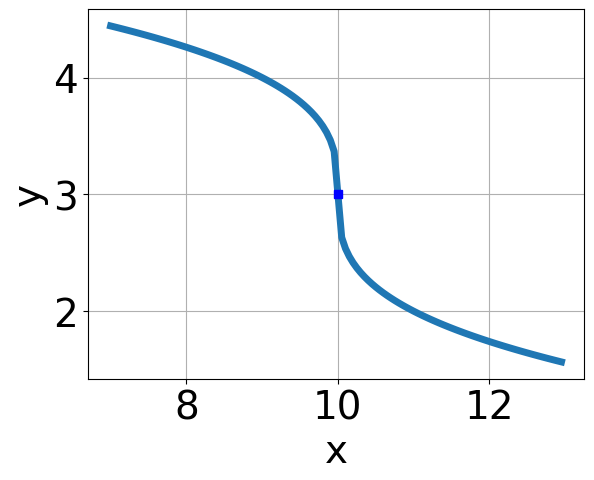
\includegraphics[width = 0.3\textwidth]{../Figures/radicalEquationToGraphAB.png}\item 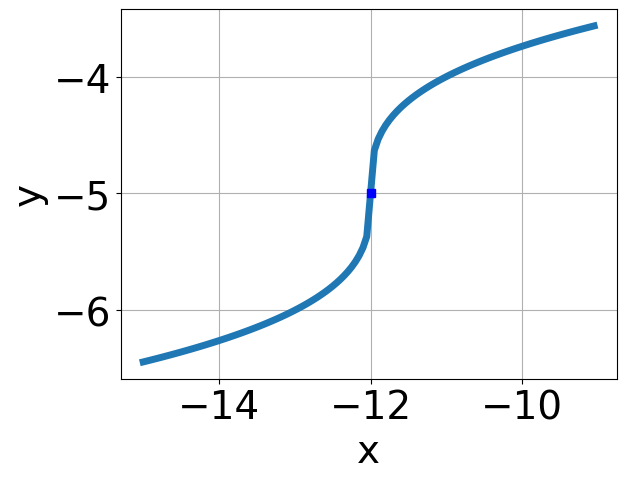
\includegraphics[width = 0.3\textwidth]{../Figures/radicalEquationToGraphBB.png}\item 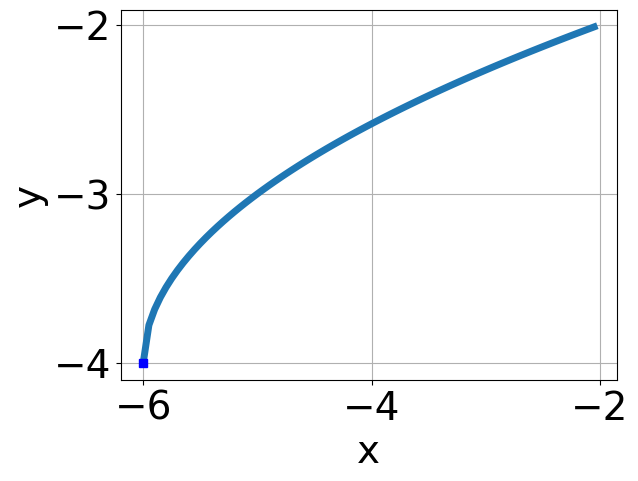
\includegraphics[width = 0.3\textwidth]{../Figures/radicalEquationToGraphCB.png}\item 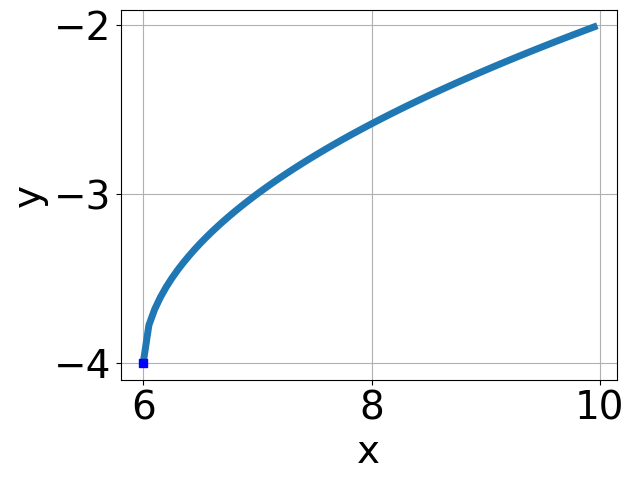
\includegraphics[width = 0.3\textwidth]{../Figures/radicalEquationToGraphDB.png}\end{multicols}\item None of the above.
\end{enumerate} }
\litem{
Solve the radical equation below. Then, choose the interval(s) that the solution(s) belongs to.\[ \sqrt{4 x - 7} - \sqrt{-8 x + 4} = 0 \]\begin{enumerate}[label=\Alph*.]
\item \( x \in [0.01,0.39] \)
\item \( x_1 \in [0.83, 1.03] \text{ and } x_2 \in [1.75,2.75] \)
\item \( x_1 \in [0.33, 0.55] \text{ and } x_2 \in [1.75,2.75] \)
\item \( \text{All solutions lead to invalid or complex values in the equation.} \)
\item \( x \in [0.83,1.03] \)

\end{enumerate} }
\litem{
Choose the graph of the equation below.\[ f(x) = \sqrt{x + 14} + 3 \]\begin{enumerate}[label=\Alph*.]
\begin{multicols}{2}\item 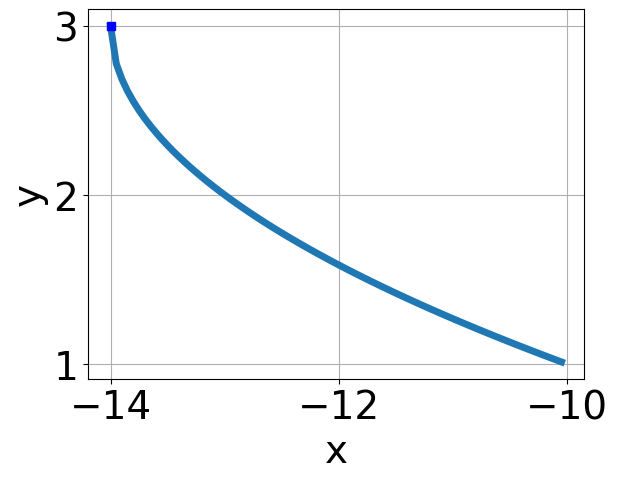
\includegraphics[width = 0.3\textwidth]{../Figures/radicalEquationToGraphCopyAB.png}\item 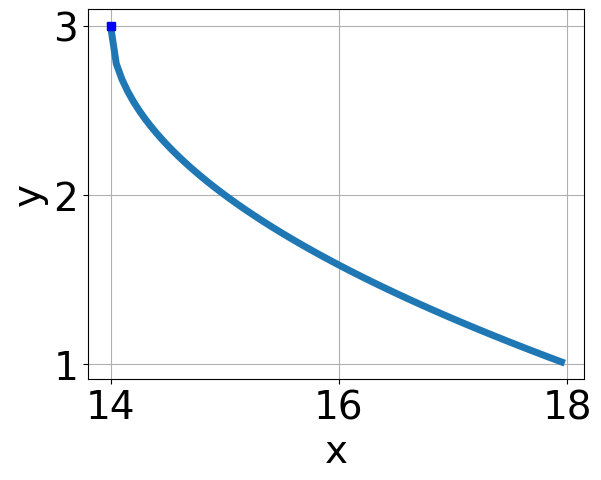
\includegraphics[width = 0.3\textwidth]{../Figures/radicalEquationToGraphCopyBB.png}\item 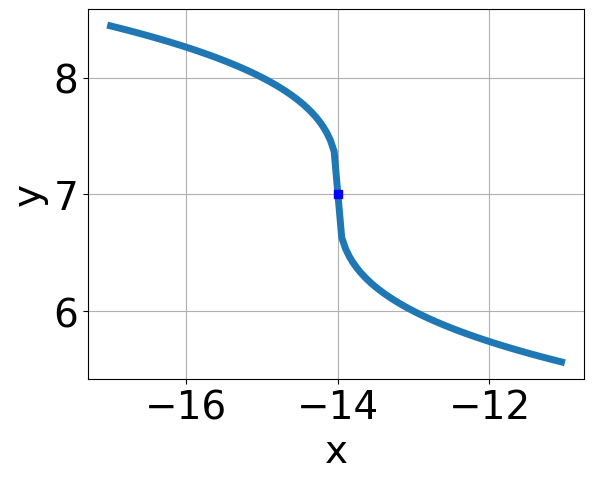
\includegraphics[width = 0.3\textwidth]{../Figures/radicalEquationToGraphCopyCB.png}\item 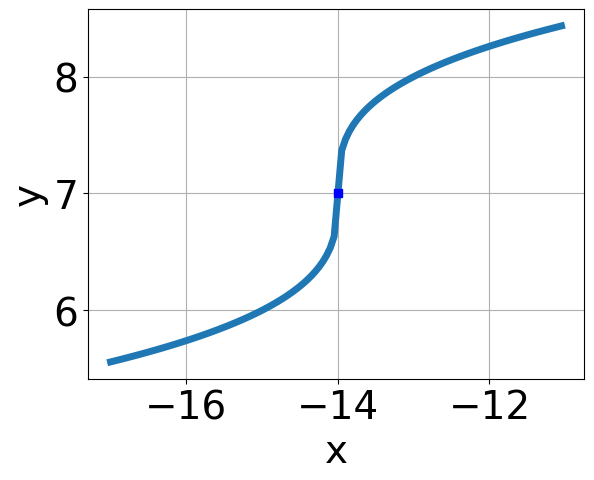
\includegraphics[width = 0.3\textwidth]{../Figures/radicalEquationToGraphCopyDB.png}\end{multicols}\item None of the above.
\end{enumerate} }
\litem{
Choose the equation of the function graphed below.
\begin{center}
    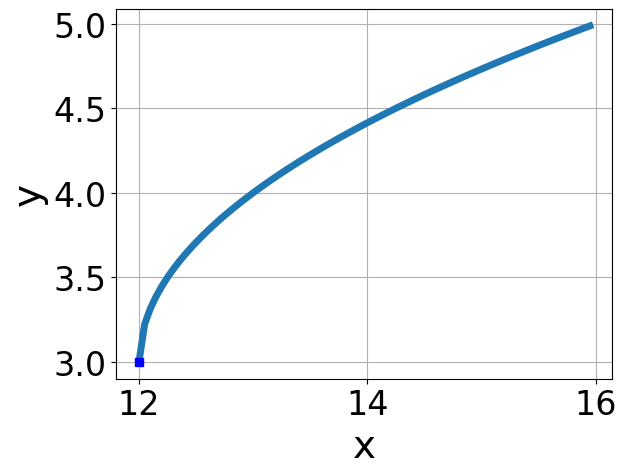
\includegraphics[width=0.5\textwidth]{../Figures/radicalGraphToEquationCopyB.png}
\end{center}
\begin{enumerate}[label=\Alph*.]
\item \( f(x) = - \sqrt[3]{x + 6} - 4 \)
\item \( f(x) = - \sqrt[3]{x - 6} - 4 \)
\item \( f(x) = \sqrt[3]{x - 6} - 4 \)
\item \( f(x) = \sqrt[3]{x + 6} - 4 \)
\item \( \text{None of the above} \)

\end{enumerate} }
\end{enumerate}

\end{document}